% TODO fill in your paper title
\newcommand{\PaperTitle}{A Comparative Analysis of Machine Learning Algorithms for Website Traffic Classification from Network Packets }
% TODO fill in your paper number when you get it
\newcommand{\PaperNumber}{XXX}

\documentclass[10pt,sigconf,letterpaper,nonacm]{acmart}

\DeclareMathSizes{12}{30}{16}{12}

%%%%%%%%%%%%%%%%%%%%%%%%%%%%%%%%%%%%%%%%%%%%%%%%%%%%%%%%%%%%%%%%%%%%%%%%%%%%
% This is the preamble; include packages as you see fit.
% Here are a few recommendations:
% \usepackage{color}
\usepackage{graphicx}
% \usepackage[labelformat=simple]{subcaption}
% \usepackage{xspace}
% \usepackage{multirow}
% \usepackage[ruled,vlined]{algorithm2e}
% \usepackage{ulem}
% \normalem

%%%%%%%%%%%%%%%%%%%%%%%%%%%%%%%%%%%%%%%%%%%%%%%%%%%%%%%%%%%%%%%%%%%%%%%%%%%%

\begin{document}

\title{\PaperTitle}

\author{Matthew Berthoud, Lake Bradford, Justin Cresent, Will Katabian}
\affiliation{
  \institution{William \& Mary}
  \city{Williamsburg}
  \state{Virginia}
  \country{USA}
}

\begin{abstract}
Accurately Identifying web traffic destination and origins is crucial for the efficiency of a network. This project explores the potential of machine learning in reference to web traffic classification based on the 
analysis of network packets. 
We monitored and analyzed web traffic data from ChatGPT, Blackboard, and Linkedin, with the objective 
of building models which will be able to predict the web traffic origin or destination of a specific packet. The collection of data was performed
using Wireshark, then the data was reformatted to eliminate bias and get more accurate results.
Using the collected data we then trained four models which had varying levels of accuracy, Logistic Regression (56\%), 
K-Nearest Neighbors (77\%), Random Forest (78\%), and finally a neural
network (84\%). This project shows the importance of machine learning within the field of 
network traffic analysis as automaton is much more efficient and precise compared to manually
examining web traffic, especially in a scale as large as the internet. One example of our project's significance is that this can be crucial data analysis 
for network administrators and security professionals, whom would examine the network for malicious traffic.

\end{abstract}

\keywords{Network Traffic, Machine Learning, Web Traffic Classification, Network Packets, Data Analysis, Neural Networks, Random Forest, K-Nearest Neighbors, Logistic Regression}

\maketitle

\section{Introduction}
The ability to monitor and analyze network traffic is crucial for the efficiency and security of a network \cite{10.1145/2388576.2388608}. 
It helps to manage the overall network performance, detect and prevent malicious activities, and ensure the network is operating as intended.
The present day internet is composed of a vast variety of diverse web traffic, of which requires a more sophisticated approach to analyze and classify network traffic\cite{10.5555/3432601.3432608}.
This project investigates a variety of machine learning algorithms to see which most accurately and effectively classify web traffic based on data from a set of captured network packets. 

  Traffic classification is very significant in practice, if done accurately and effectively \cite{10.1109/TNET.2014.2320577}. For reasons mentioned previously, the observed capabilities of this and other projects 
  can be crucial for network administrators and security professionals, whom would examine the network for malicious traffic.

  For this project, many sets of packet data were collected from three popular websites: ChatGPT, Blackboard, and Linkedin. These sets were then merged into a single dataset, which was then split into training and testing sets. 
  Four models were then trained and tested on this data: Logistic Regression, K-Nearest Neighbors, Random Forest, and Neural Network \cite{scikit-learn}. 

  A thorough evaluation of the models was conducted through testing and validation sets, hyperparameter optimization employing cross-validation and grid search, and computing accuracy and Macro F1 scores. The results showed that the Neural Network model 
  acheived the highest accuracy of $84\%$ and Macro F1 score of { \bf BLANK}. %%TODO fill in the score.%%
  These scores display the model's ability to accurately classify the selected websites based on captured network packet data.

  Overall, the significance of this project is seen in its use of Machine Learning and the extensions of these applications into the discipline of network traffic analysis. This practice has potential to be utilized in real-world applications, and many sources
  prove it already is \cite{10.5555/3432601.3432608}. 

\section{Proposed Method}
This section presents the methodology for how this project goes about capturing network packet data, analyzing the data, and classifying it based on its website of origin.

\subsection{Capturing Data}

\begin{figure*}[t]
  \centering
  \includegraphics[width=\textwidth]{Figures_and_Graphs/webCollectionDiagram.png}
  \caption{Wireshark Data Collection Process}
  \label{fig:dataCollection}
\end{figure*}
\begin{figure*}[t]
  \centering
  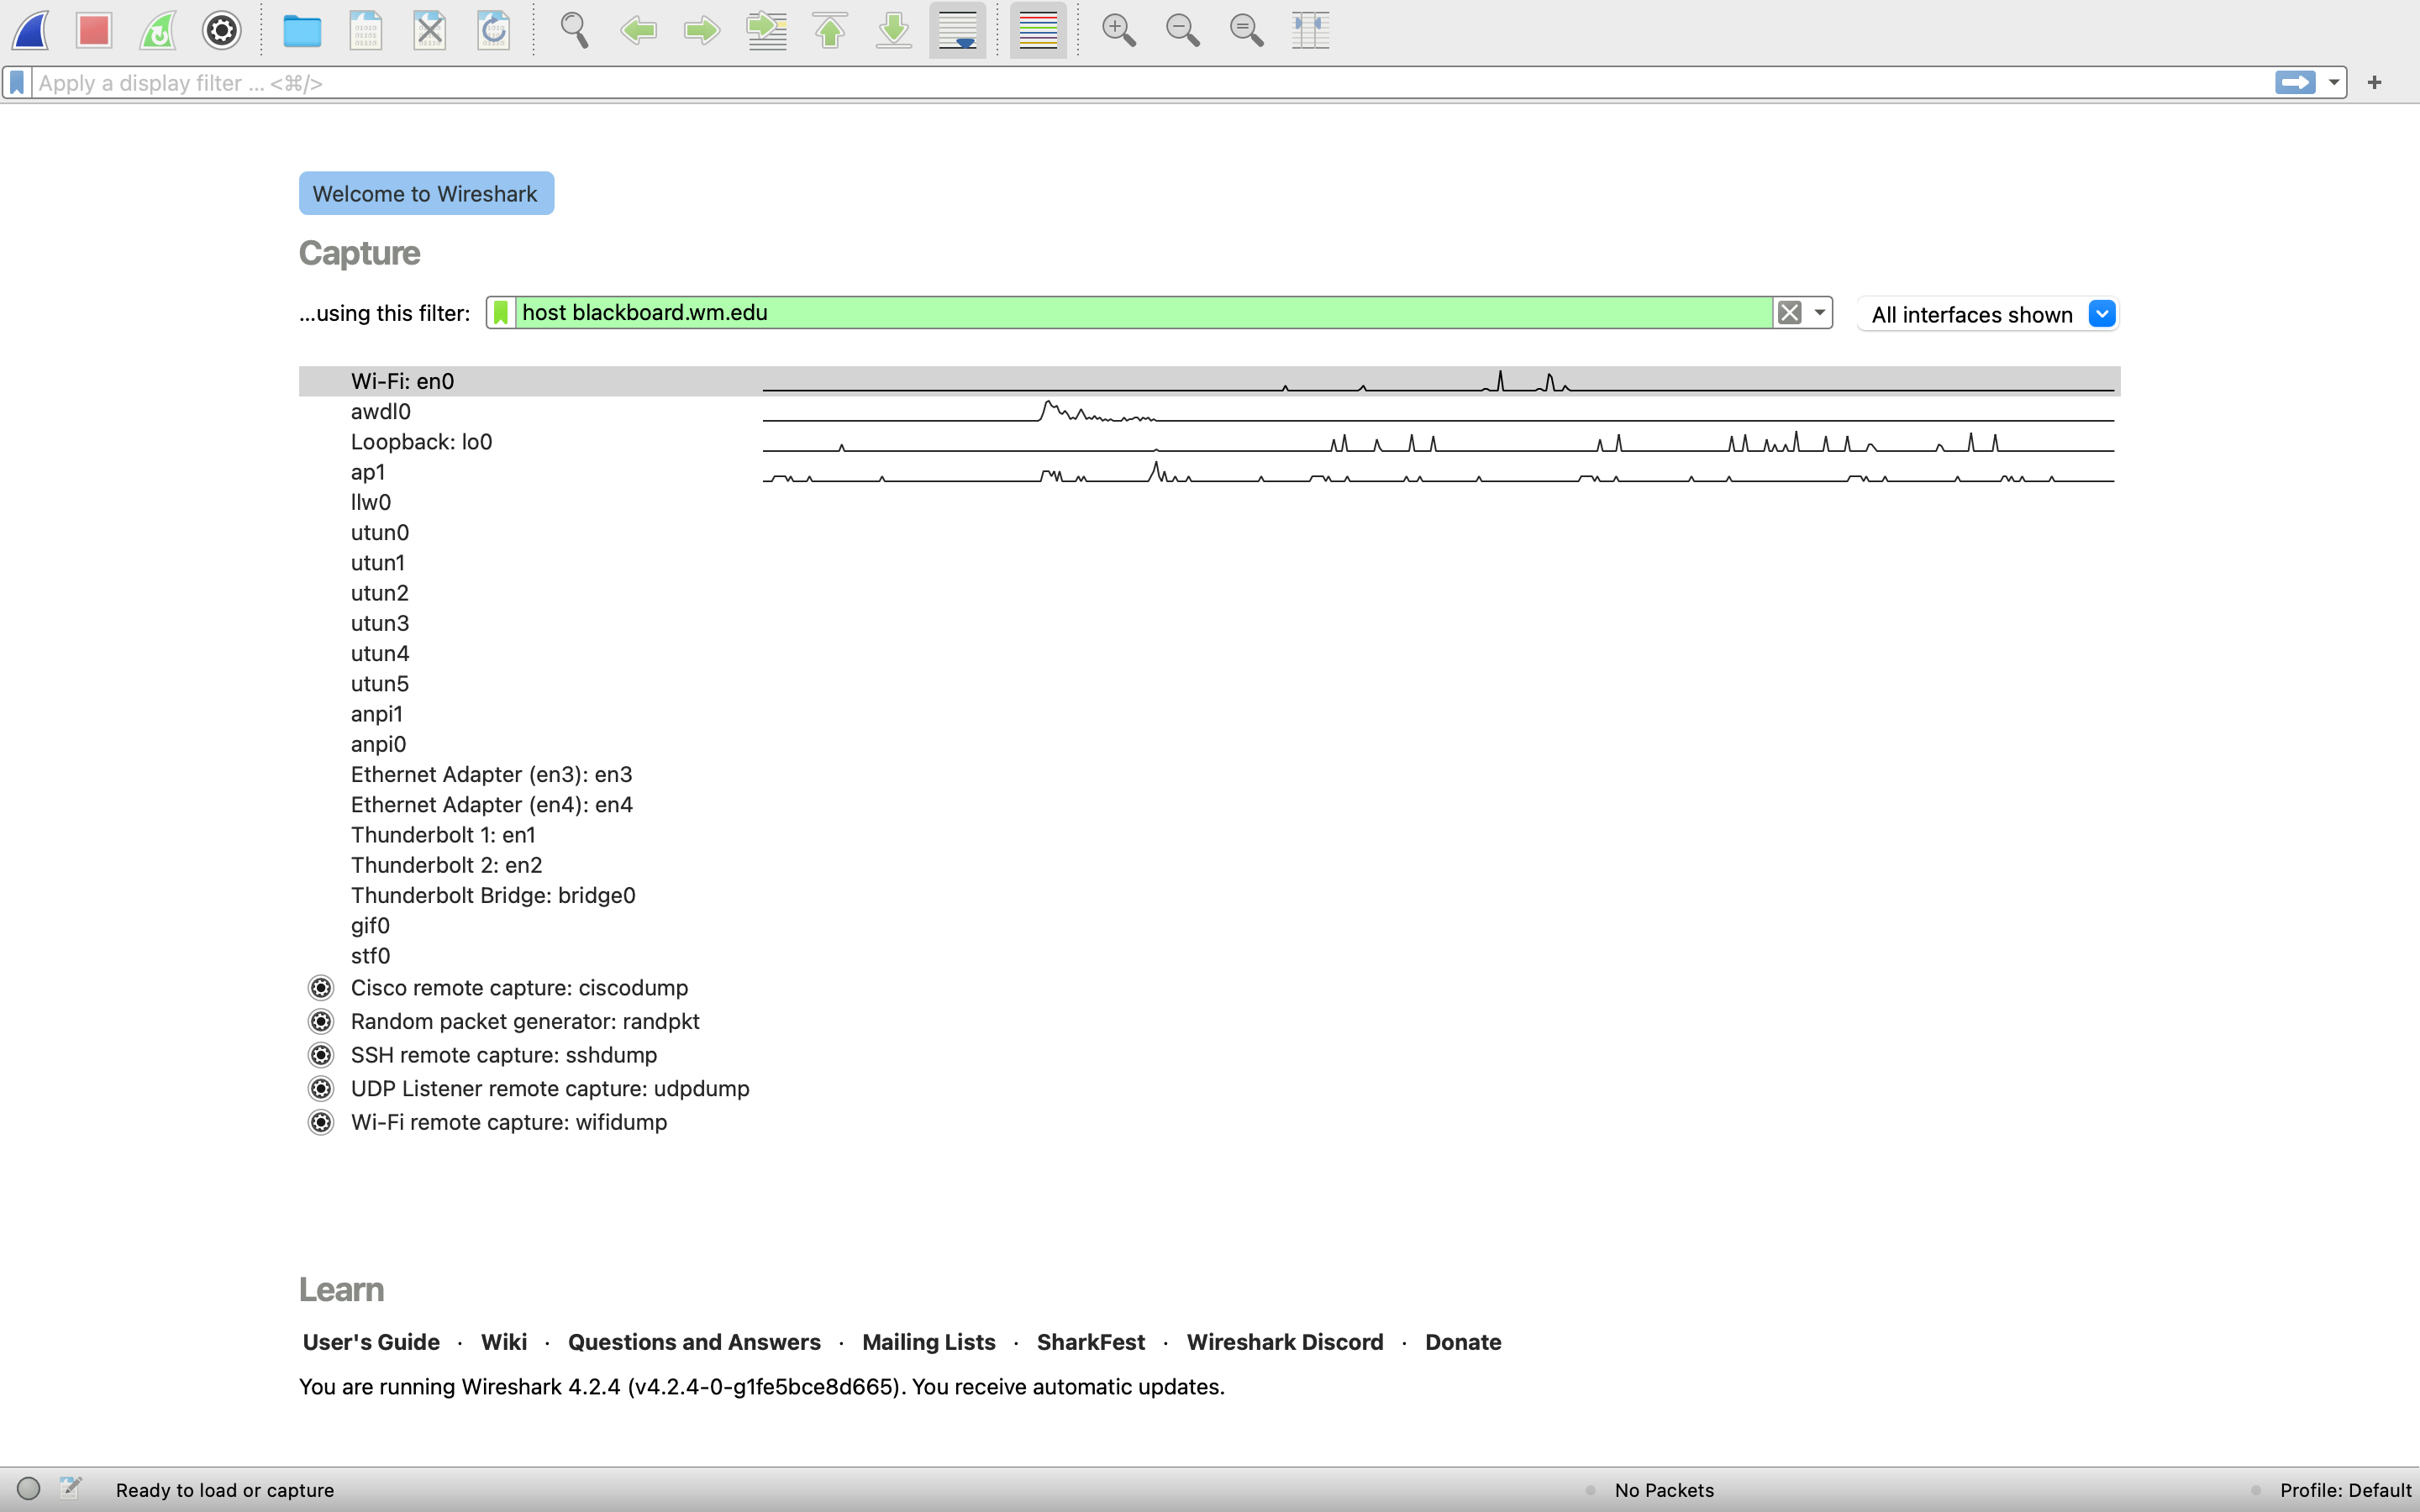
\includegraphics[width=0.72\textwidth]{Figures_and_Graphs/wiresharkFigure.png}
  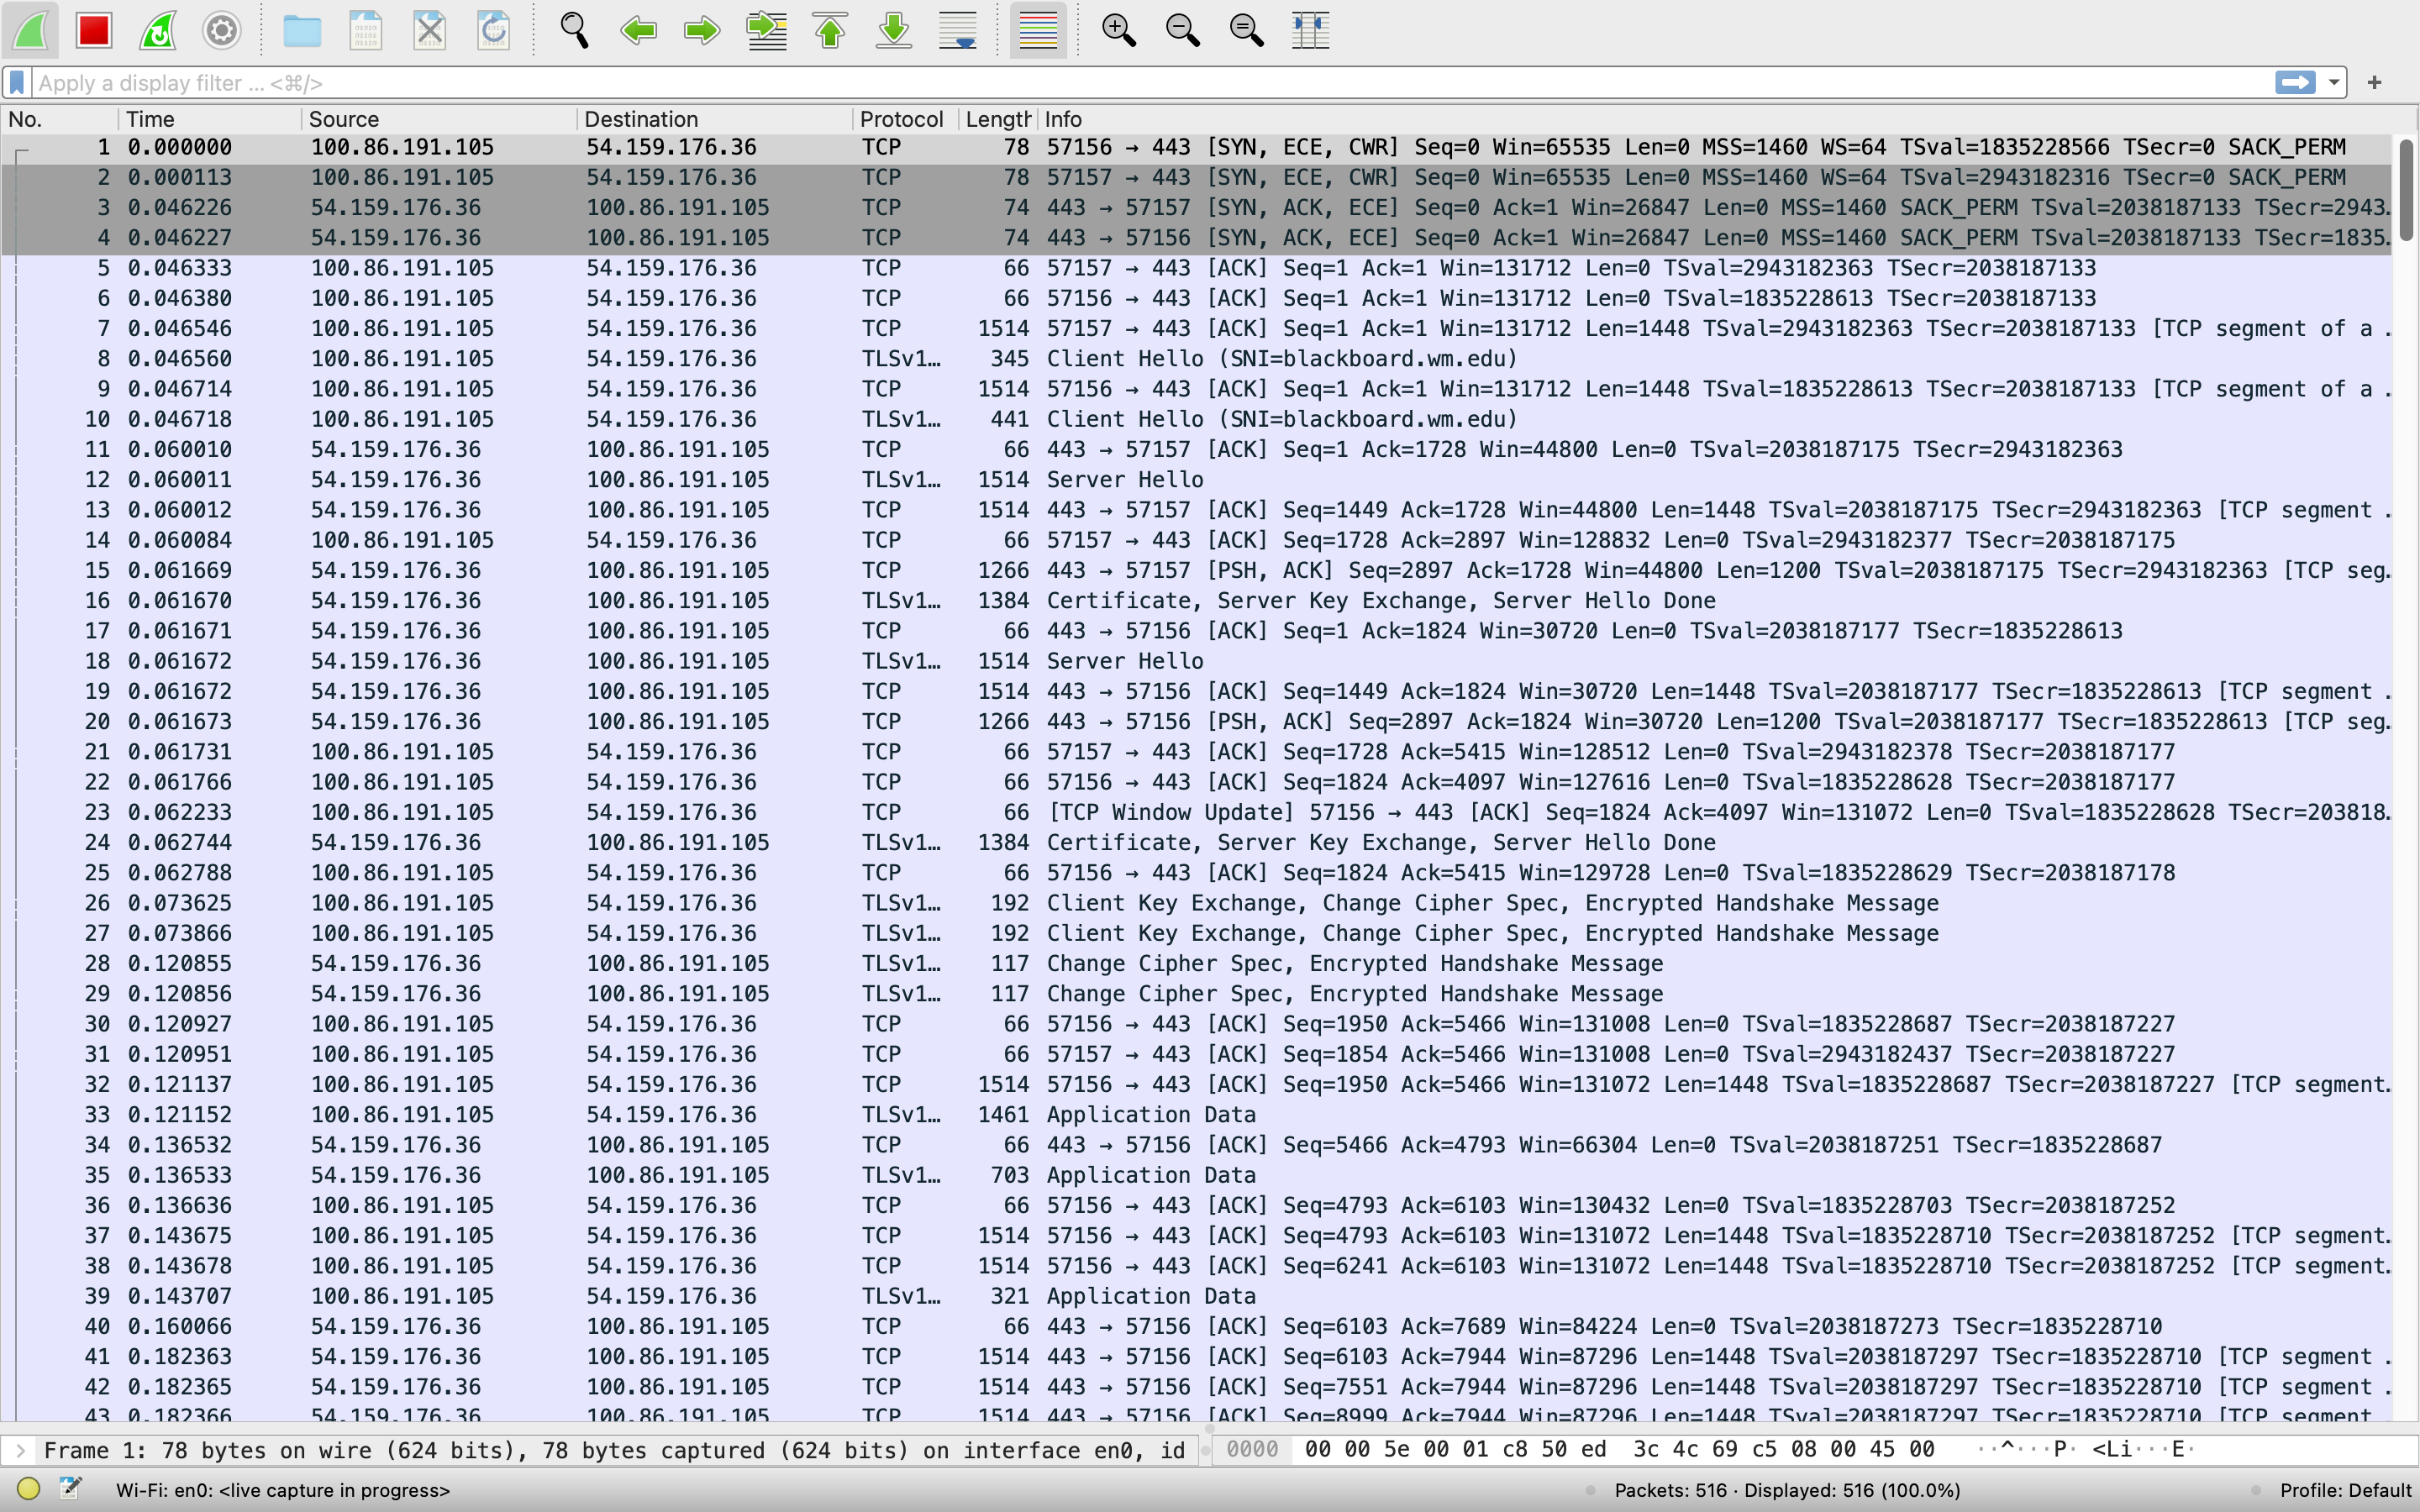
\includegraphics[width=0.73\textwidth]{Figures_and_Graphs/wiresharkDataFigure.png}
  \caption{Wireshark interface and example of captured data}
  \label{fig:wireshark}
\end{figure*}
\subsubsection{Network analysis tool} For this project, the tool chosen and used was Wireshark \cite{Wireshark}, a widely used network protocol analyzer. Wireshark is capable of capturing and analyzing network packets, and is able to provide a detailed
 view of the packets exchanged between the client and server. Wireshark offers a broad variety of features that allow for users to capture, decode, and analyze network packets. It shows the packet data in a human-readable format, and provides a detailed view of the packet's contents.
 This data contains information on time taken for packet to send and arrive, protocols used, size of each packet, and other fields such as more information on the packet and the source IP address. This tool also supports use of different forms of link communication and can be specified to capture packets from a specific network interface (ie. Ethernet, Wifi, etc.). 
 The many applications and ease of use of Wireshark make it a great tool for this project.
 
 The process for this project (shown in figure \ref{fig:dataCollection}) involved setting a hostname filter for each desired website, capturing packets from the host, and then exporting the data to a CSV file.

 \subsubsection{Data Collection}
To commence the collection of our data, we open Wireshark and select a network connection. 
In this project we established a connection the College of William and Mary's network interface (en0). In order to isolate the web traffic in order to specifically collect 
packets that we are analyzing, the capture filter functionality is utilized. The website of interest is then visited in the web browser which causes Wireshark to begin collecting the packets being exchanged.
After collecting sufficient packets, the data is then converted into a Comma Separated Values (CSV) file. This process of data collection is performed for Blackboard, LinkedIn, and ChatGPT resulting in the creation of 
three distinct files. 

\subsection{Data Preparation and Processing}
In order to ensure the integrity and reliability of our models,
the collected data must be processed prior to model training.


\subsubsection{Feature Selection}
The data collection process using Wireshark yields a dataset containing seven distinct features shown in figure \ref{fig:wireshark}. 
\begin{itemize}
  \item \textbf{Packet Number}: An integer representing the order in which the packets were captured during the Wireshark session. Provides insight on the order of the packets on the network interface. 
  \item \textbf{Time}: A floating point value representing the relative timestamp for each packet since the start of the Wireshark session. Similar to packet number, the time feature provides a better understanding of the packet order yet is more precise.
  \item \textbf{Source}: A string value containing the internet protocol address of the device that the packet originated from. 
  \item \textbf{Destination}: A string value containing the internet protocol address of the device that is receiving the packet. 
  \item \textbf{Protocol}: A string value which contains the network protocol employed for the transmission of the packet. Three distinct protocols were identified within the datasets used in this project (QUIC, TCP and TLSv1.2).
  \item \textbf{Length}: An integer representing the size of a packet in bits 
  \item \textbf{Info}: A string value containing more information pertaining to a packet. This value can vary heavily between packets.
\end{itemize} 
As the objective of this project is to predict the origin of web traffic, both source and destination are excluded from the dataset used to train the models. 
Including these would be of course the simplest way to classify the data, of course, but the objective of this investigation is to have a highly applicable mechanism to classify network data when a small subset of information is available. 
Including the dependent variable of the research question as an independent variable would trivialize the research.

The info feature is also removed from our data, since its meaning highly varies from packet to packet. Two example Info fields are shown below:

Example 1:
\begin{verbatim}
"Protected Payload (KP0)"
\end{verbatim}

Example 2:
\begin{verbatim}
"Initial, SCID=01d117623d73ec3a2fd3
9d62da73e7cc7e63ff11, PKN: 0, ACK"
\end{verbatim}

There is no good reason to think this would help with classification, and even if it were to improve the accuracy with our test set, we have no ability to predict in good faith that this would always be the case, since there isn't a consistent semantic meaning.

Consequently, the features selected for training and testing the models are Time, Length, and Protocol. The Protocol feature is converted to an integer for compatibility with 
the models using a dictionary to map protocol names to a corresponding numerical representation (e.g., \texttt{TCP}: 0, \texttt{QUIC}: 1, \texttt{TLSv1.2}: 2) as shown in figure \ref{fig:webTraffic}.  Additionally, a categorical variable titled "Website" 
is created which displays which website the packet originated (e.g., LinkedIn, ChatGPT, Blackboard). The "Website" feature acts as the target variable and allows 
the models to detect relationships between the packets and their corresponding web traffic origin. 

\subsubsection{Data Formatting}
To maintain normalized representation in all the collected datasets, a process of data harmonization 
was applied after collecting the necessary data. The dataset with the minimum number of observations is identified and accounted for when
truncating the remaining two datasets. Subsequently, the three datasets are combined and rearranged to minimize bias while training each of our models.
This process ensures a balanced yet unbiased dataset that maximizes the effectiveness of our models. Figure \ref{fig:webTraffic} presents the refined data following the data preparation. 

\begin{figure*}[htp] 
  \centering
  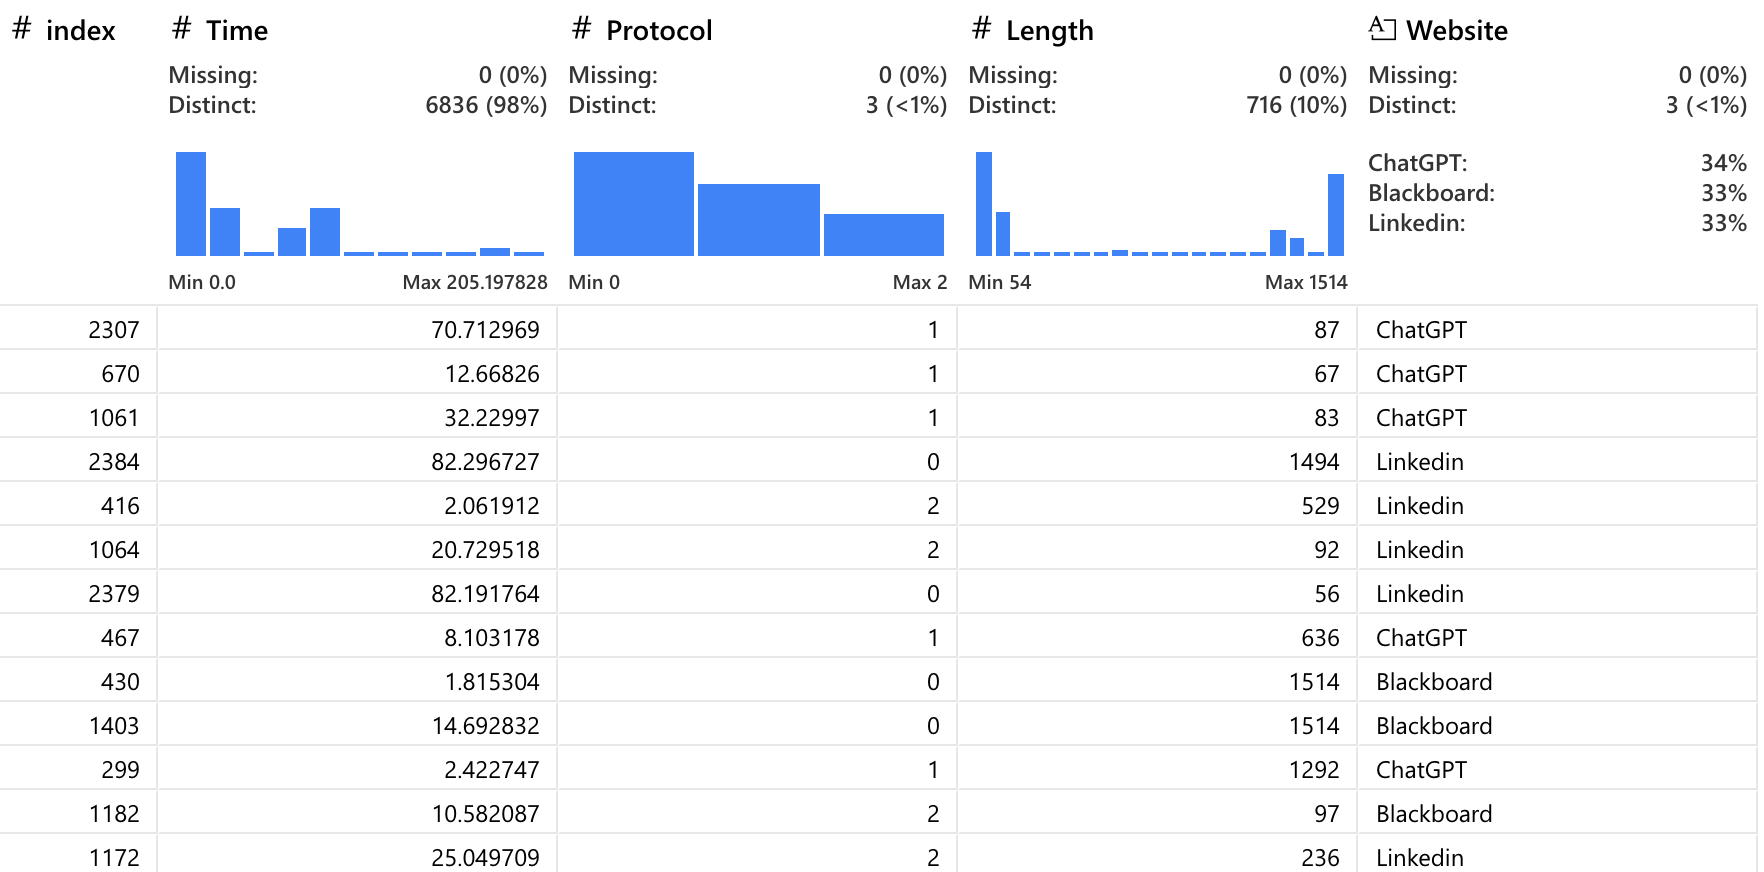
\includegraphics[width=\textwidth]{Figures_and_Graphs/fullDataDiagram.png}
  \caption{Processed Web Traffic Data}
  \label{fig:webTraffic}
\end{figure*}

\subsection{Employed models}
For this project, we required a classification model that would be able to accurately predict the website of origin for a given packet. In the end, we chose to employ four different models: Logistic Regression K-Nearest Neighbors, Random Forest, and a Neural Network.
The reason we selected more than one model was to be able to effectively compare the performance of each and determine which was the most effective for our solution.
We tested the models sequentially, learning lessons along the way about the format of the data, and what similarities and differences exist in the data that could be potentially exploited by a subsequent model.

\subsubsection{Logistic Regression (Baseline)}
As a starting point, we employed the Logistic Regression model as a baseline for our data analysis. Logistic regression is a statistical method used for binary classification tasks, where the goal is to predict the probability of an event happening or not happening.
It was understoof initiallly that this model may not be an ideal fit for our data; due to the regressions binary nature having more than two classifications is not ideal.

Characteristics of Logistic Regression:
\begin{enumerate}
  \item \textbf{Binary Outcome}: Logistic regression is used for binary classification tasks, where the outcome variable has only two possible outcome
  \item \textbf{Linear Relationship}: Logistic regression assumes a linear relationship between the independent variables and the log-odds of the outcome
  \item \textbf{Probablistic Output}: Instead of predicting discrete classes directly, logistic regression predicts the probability that a given observation belongs to a particular class
  \item \textbf{Interpretability}: Logistic regression coefficients represent the change in the log-odds of the outcome for a one-unit change in the corresponding independent variable, making it easy to interpret the impact of each variable on the outcome. This characteristic was especially important for our baseline
\end{enumerate}

The Logistic regression was such an ideal choice for our baseline specifically because of its interpretability characteristics. We wanted to pick a model which would $(1)$ allow us the swiftest entry point into our approach and $(2)$ allow for us to not only have a simple foundation but a foundation from which we could improve upon.

The execution of this model was rather simple: splitting the data into training and testing sets and executing a standard regression to be analyzed. This simplistic approach, as previously mentioned, allowed for us to inspect which features were most advantageous for us and more importantly which features we would continue to analyze.

\begin{figure}[h!]
  \centering
  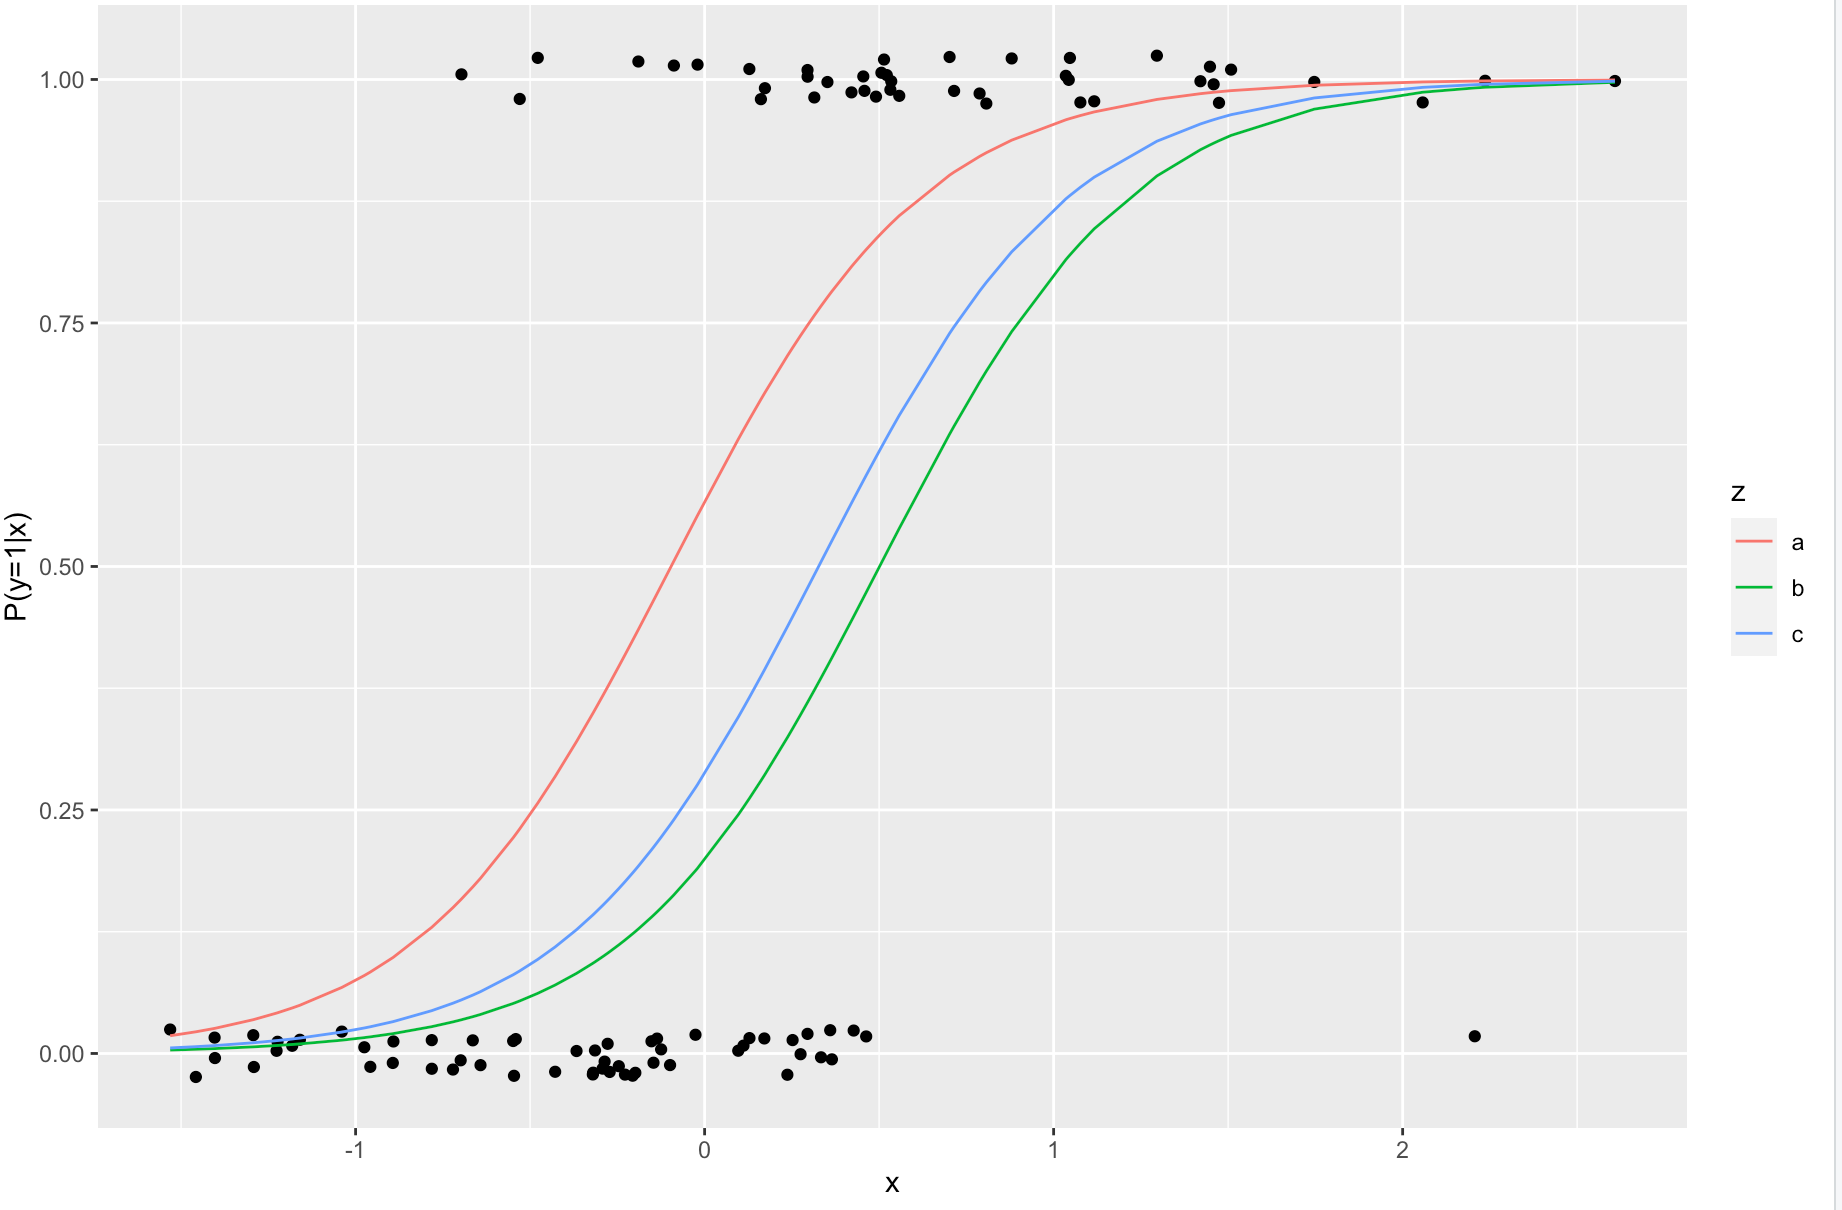
\includegraphics[width=9cm]{Figures_and_Graphs/LogReg.png}
  \caption{Logistic Regression model structure example}
  \label{fig:RFExample}
\end{figure}

\subsubsection{K-Nearest Neighbors}
K-Nearest Neighbors (KNN) is a supervised learning model which classifies data points
based on their proximity to a specified number (k) of existing data points.
\begin{figure}[htp] 
  \centering
  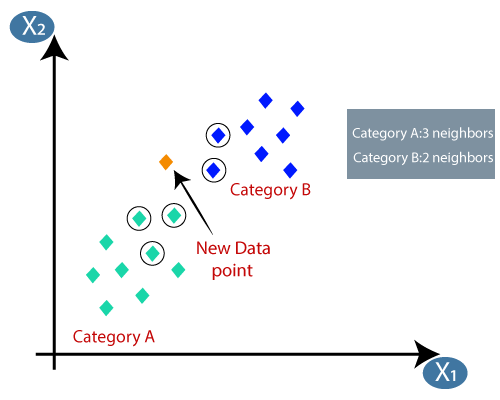
\includegraphics[width=0.5\textwidth]{Figures_and_Graphs/knnExample.png}
  \caption{K-Nearest Neighbor model structure example}
  \label{fig:ExampleKNN}
\end{figure}

The implementation process is as follows: 
\begin{enumerate}
  \item \textbf{Optimization and Training}: Prior to training the model, the optimal number of neighbors (k) for the model is identified using K-Fold cross validation. This technique involves dividing the training data into multiple folds and utilizing one fold for validation while the remaining ones are used for training. For every fold, a KNN model is trained with a specified k value and the accuracy (external validation) is calculated. Multiple different k values are tested using this process and the k value that yields the highest average external validation is used in the final model. After the optimal k value is calculated, the model achieved an accuracy of 97\% on the training data. 
  
  \item \textbf{Evaluating Model}: In order to assess the effectiveness of the model, an independent dataset containing 2000 packets was collected and evaluated. Having the model evaluate a separate unseen dataset reveals a more realistic measurement of the accuracy of our model. After evaluating this dataset, the KNN model achieves an accuracy of 77\%.
\end{enumerate}

\subsubsection{Random Forest}
A Random Forest is a form of an ensemble model that is composed of multiple decision trees. Each tree is ran and gives its predicted classification, and the final classification is determined by a majority vote of all the trees (seen in figure \ref{fig:RFExample}).

Advantages of Random Forest Models:
\begin{enumerate}
  \item \textbf{Ability to handle complex features}: Random forests have the ability to handle complex features, such as time and protocols in the case of network packets, and the relationships between them, which can be very important in classifying network traffic.
  \item \textbf{High accuracy}: Random forests diminishes the problem of overfitting that can occur in decision trees, and can achieve higher accuracy, helping to more accurately determine website origins of a packet.
  \item \textbf{Feature importance}: Random forests can provide insight into which features are most important in the classification process, such as protocol vs time in classifying websites for this project.
  \item \textbf{Scalability}: Random forests can be scaled to handle much larger datasets, which can be very important for network traffic which can receive a high volume of packet data extremely quick.
\end{enumerate}

\begin{figure}
  \centering
  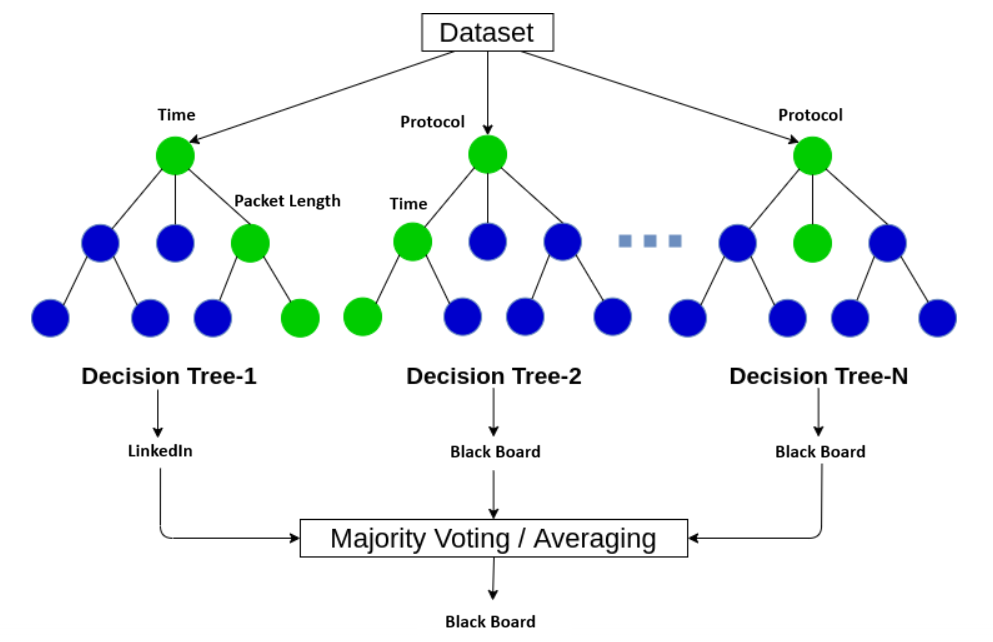
\includegraphics[width=9cm]{Figures_and_Graphs/RandomForestExample.png}
  \caption{Random Forest model structure example}
  \label{fig:RFExample}
\end{figure}

The library used for the Random Forest model was scikit-learn \cite{scikit-learn}. Sci-kit learn's implementation of Random Forests utilize aggregation to take a soft vote of the soft classifications (probability of the packet being from each class). Within soft voting, a weighted average of the probabilities from the classification are taken, and the class with the highest probability is chosen as the final classification.


\subsubsection{Neural Network}

The final model we chose to use was a Neural Network.
A Neural Network is a machine learning model that tries to make decision as if it were a human brain. 
It consists of a graph of nodes, analogous to neurons, that are interconnected by directed edges, analogous to synapses.

The nodes are organized into layers, as specified here.
\begin{enumerate}
    \item {\bf Input Layer}: The input layer is, as it sounds, the interface through which the independent variable data comes into the model. 
    In our case, since the model had three inputs, Time, Length, and Protocol, there were three nodes in the input layer.
    \item {\bf Output Layer}: The output layer is the layer that makes the decisions as to what classes the data are places in. In a "one-hot-encoding" scheme, which is what we employed, there are as many nodes as there are output classes in the data. For our purposes, this corresponds to three nodes, one for Blackboard, one for ChatGPT, and one for LinkedIn. One of the nodes is activated for each data point, and that is the class label it receives.
    In binary classification data sets, you could use a single node, and define a threshold, before which the output is classified as class 0 and after which the output is classified as class 1.
    We could have done something similar, by having two thresholds, where either end of the distribution classifies into one of two classes, and the middle classifies into a third, but we felt that the one-hot method made more sense for a number of reasons.
    Namely, the activation functions available (touched on later) didn't provide adequate separation for the simplistic data we have, 
    and the middle class being between two thresholds while the other two are open ended is an unfair and unnecessary bias.
    \item {\bf Hidden Layer(s)}: The input and output layers can be directly connected by edges. 
    This, if fully connected, would be called a perceptron. 
    You'll recall our model, however, is called a multi-layer perceptron. 
    This is because there are some $n$ hidden layers, with $m$ nodes each, connected to one-another between the input and output layers.
\end{enumerate}
\begin{figure}
    \centering
    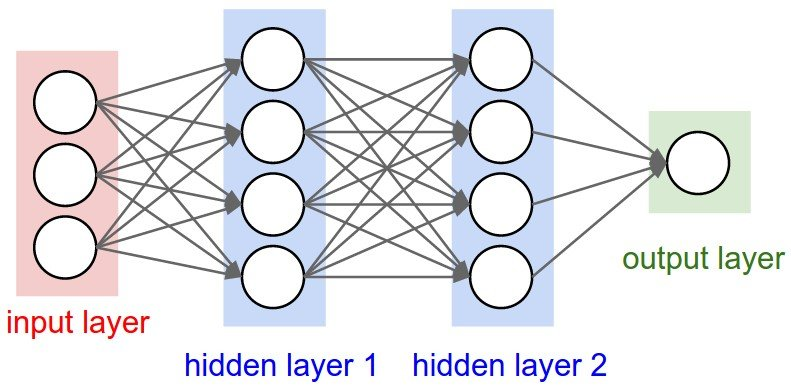
\includegraphics[width=1\linewidth]{Figures_and_Graphs/nn_example.png}
    \caption{Neural Network Model Structure Example}
    \label{fig:nn}
\end{figure}

In a fully-connected neural network, or multilayer perceptron (MLP), which is what our model used, all of the nodes in each layer of the topology are connected to every node in the next layer, and every node in the previous layer. Nodes at the same layer are not connected.

The resulting graph structure is directed, meaning each edge moves in one direction, away from the input layer and towards the output layer. Figure 
\ref{fig:nn}
shows the topology and edge structure of an MLP with a 3 node input layer, like out model, a 1 node output layer, {\it unlike} our model, and two hidden layers with four nodes each.

Any given node is related to the connected nodes in the following way.
Say node $Y$ represents a node in the first hidden layer of Figure \ref{fig:nn}.
There are 3 inputs from the input layer: $x_1, x_2, x_3$, and four required outputs, all of which will be the same . Within the node, The three inputs are fed into this equation:

$$z = \sum_{i=1}^3(x_i \cdot w_i) + b$$

Variables $w_i$ and $b$ correspond to weight and bias, respectivly. Both of these terms get set by the training process of the model, which we'll discuss shortly. 
The resulting value, $z$, is the input to an {\it activation function}, which, depending on which is used, modifies and normalizes the output before it is passed to the next node. 

$$output = activation(z)$$

After activation, the math at this node is finished, and the post activation output becomes the input from this node for all the nodes in hidden layer 2.

Through a solving process, the specific algorithm of which (lbfgs) will be passed into the model, 
the weights and bias are all calculated for every node, in order to maximize accuracy.

These mathematical procedures would be heavily skewed by outliers in the dataset. Therefore, we made the choice to scale the data using ski-kit-learn's \texttt{Standard Scaler} class to scale all the data between 0 and 1.

Hyperparameters to a neural network define how it is built. We tuned these extensively, in multiple grid searches. The settled-upon hyperparameters include:

\begin{enumerate}
    \item {\bf Activation function}: Logistic. The logistic, or sigmoid activation function shapes the input features into a binary output. This is necessary at each layer, as well as for one-hot encoding.
    \item {\bf Alpha (learning rate)}: $\alpha = 0.1$. This is an input to the Solver function, which helps to determine the rate at which the model learns.
    \item {\bf Hidden Layer Sizes}: 1 layer of 20 nodes. 
    \item {\bf Solver}: Limited memory Broyden-Fletcher-Goldfarb-Shanno (lbfgs) algorithm. This is the quasi-Newton method by which the weight and bias hyperparameters are tuned. 
\end{enumerate}

As mentioned, these hyperparameters were not chosen at random. We ran a GridSearch on many possible combinations of parameters, exhaustively searching every combination. In order to do this, we used the \texttt{GridSearchCV} library in python from scikitlearn, which allowed us to divide the training data into 5 partitions. Then 5 separate times, each of the partitions could be used as the validation data, while the rest of the training data was used to solve the network. These 5 models were bulilt for every possible combination of hyperparameters, from the input hyperparameters shown below.

\begin{verbatim}
parameters = {
    'activation': ['identity', 'logistic', 
                    'tanh', 'relu'],
    'solver': ['adam','lbfgs','sgd'],
    'alpha': 10.0 ** -np.arange(-1, 10),
    'hidden_layer_sizes':[(10),(12),(14),
                          (16),(18),(20)]
}
\end{verbatim}

After running this grid search, we calculated the validation accuracy from every model, and mean validation accuracy within the 5 folds for each set of hyperparameters. The highest validation score and therefore model we chose, was $.94$. 
Then, we rebuilt that network and scored it on the fully separate test data. We'll discuss results from the test data in the next section.

\section{Evaluation}
This section comprehensively evaluates our models and their performance on the dataset and validating sets. Later, goes on to determine the model which best classified our selected websites based on network packet data.

\subsection{Dataset}
Our dataset of packets acquired from wireshark was split up in a couple of ways. First and foremost, we had completely separate training data and test data. The training data was used in training processes such as KFold validation that require it to be split "test"-train splits, but we refer to those "test" sets as validation sets, because they are part of the training process, and completely unrelated to the test data.

Moreover, we used the same test data on all four models, in order to ensure an accurate comparison between them, since their performance is therefore measured with similar constraints.
We also used the same training data for all four models, except in the Neural Network we collected and added additional data. This is because Neural networks tend to need more data on which to train.

\subsection{Evaluation Metrics}
Accuracy and Macro F1 score were the primary metrics used to evaluate each model. 

These metrics are applicable to all models and allow for
a direct comparison for each of their performances. Two other metrics: precision and recall, help to provide a more detailed understanding of the model's performance on a class-to-class basis.
\newline \\
The equation for \textbf{Accuracy}: \\
\[
Accuracy= \frac{TP + TN}{TS}
\]
\newline \\
The equation for \textbf{Macro F1}: \\
\[
Macro F 1= \frac{1}{n} \sum_{1}^{n} \frac{2*Precision_i*Recall_i}{Precision_i+Recall_i}
\]
\newline \\
The equation for \textbf{Recall}: \\
\[
Recall= \frac{TP}{TP + FN}
\]
\newline \\
The equation for \textbf{Precision}: \\
\[
Accuracy= \frac{TP}{TP + FP}
\]
\\
Accuracy straightforwardly measures the probability of correctly identifying a packet based on the rate at which packets are correctly classified in the validation or test sets.

Macro F1 is more opaque in terms of being intuitively understood, but it's a harmonic average of each class's metrics of precision and recall, averaged across all classes

Recall is the calculation of how many classifications the model got correct for a given class, out of the total number of packets truly from that class.

Precision is the calculation of how many classifications that were marked as as class truly belong to each class.

\subsection{Model Comparison and Evaluation Results}
The results in table \ref{tab:results} show that the neural network achieved the highest accuracy (85\%) and Macro F1 score {\bf BLANK}. These results mean the model was the most effective at classifying the selected websites based on network packet data.
This displays that the neural network is more effective at representing complex relationships in the data than the other models. 

The logistic regression has the lowest scores by far. This makes sense, since it was a dataset with 3 dependent variable classes, and logistic regression is a binary classifier. 
The model wasn't designed for this task, so a low accuracy makes sense.

{\bf include logreg scatterplot and actual scatterplot here}

As you can see from the scatterplot, 

{\bf yap about scatter plots}

Beyond the baseline logistic regression model, the other models all perform fairly similarly, in the high 70s and low 80s in terms of test accuracy.
These numbers are good, but not great, for a number of reasons.

First, as you can see from the Actual sample space scatter plot, there is a lot of clustering of the data, particularly in terms of the Protocol feature. ChatGPT uses almost exclusively QUIC protocols, whereas Blackboard and LinkedIn use a mix of TCP and TLSv1.2. This makes differentiating chatGPT from either of the others trivially easy, but disambiguating Blackboard and LinkedIn relatively hard.

You'll notice in the heatmaps in figures \ref{knn_heatmap}, \ref{rf_heatmap}, and \ref{nn_heatmap} that chatGPT is classified 100\% accurately by RF and NN, and is very close with KNN. 

\begin{figure}
    \centering
    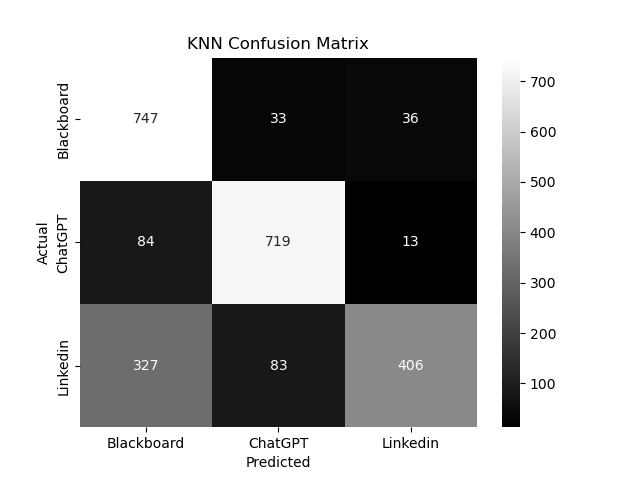
\includegraphics[width=1\linewidth]{Figures_and_Graphs/ConfusionMatrixKNN.png}
    \caption{K Nearest Neighbors Model Heatmap}
    \label{fig:knn_heatmap}
\end{figure}

\begin{figure}
    \centering
    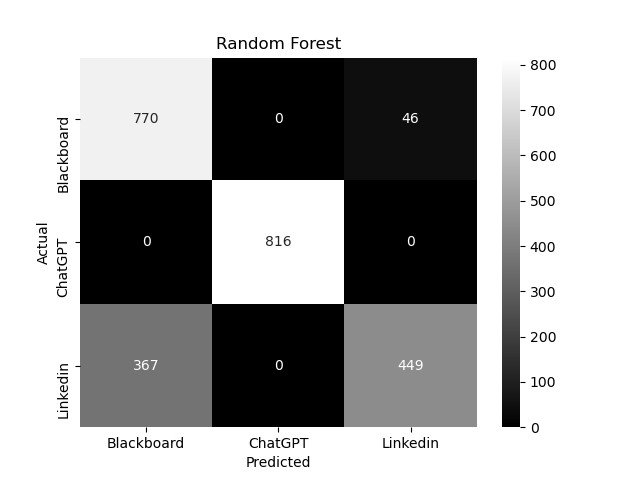
\includegraphics[width=1\linewidth]{Figures_and_Graphs/ConfusionMatrixRF.png}
    \caption{Random Forest Model Heatmap}
    \label{fig:rf_heatmap}
\end{figure}

\begin{figure}
    \centering
    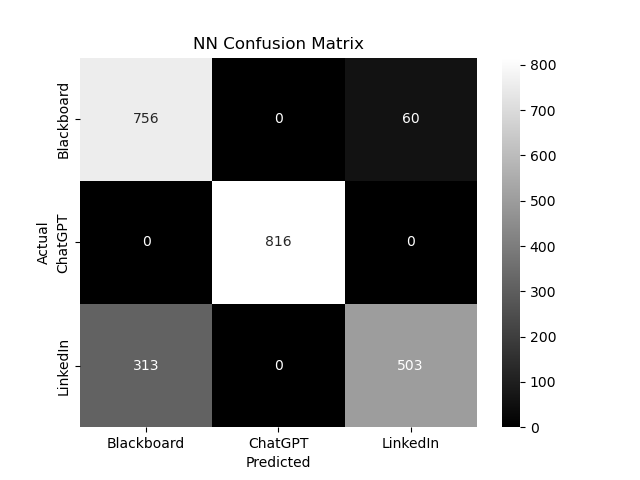
\includegraphics[width=1\linewidth]{Figures_and_Graphs/ConfusionMatrixNN.png}
    \caption{Neural Network Model Heatmap}
    \label{fig:nn_heatmap}
\end{figure}

If all of our packets had their own protocols, we'd probably be able to use a simple decision tree with two splits and get nearly 100\% accuracy.
In reality, the physical closeness of LinkedIn and Blackboard data made it hard for KNN to accurately guess based on neighbors, for the Random Forest to build meaningfully effective trees, and for the Neural Network to solve itself cleanly.

{\bf Do some data analysis to see what feature WAS useful for distinguishing BB and LI.}

  \begin{table}[!h]
    \begin{center}
    \caption{Accuracy and Macro F1 Scores for Each Model}
    \label{tab:results}
    \begin{tabular}{|c|c|c|}
      \hline
      Model & Accuracy & Macro F1 \\
      \hline
      Logistic Regression & 56\% & 0.00 \\
      K-Nearest Neighbors & 77\% & 0.00 \\
      Random Forest & 83\% & 82\% \\
      Neural Network & 85\% & 0.00 \\
      \hline
    \end{tabular}
    \end{center}
  \end{table}

\section{Discussion \& Future Work}
\subsection{Analysis of Results}
\subsection{Future Work}

\section{Conclusion}

% Note from the CFP that this section must include a statement about
% ethical issues; papers that do not include such a statement may be
% rejected.

%%%%%%%%%%%%%%%%%%%%%%%%%%%%%%%%%%%%%%%%%%%%%%%%%%%%%%%%%%%%%%%%%%%%%%%%%%%%
% We're in the endgame now

\bibliographystyle{ACM-Reference-Format}
\bibliography{refs}
\cite{10.1145/2388576.2388608}
\cite{10.5555/3432601.3432608}
\cite{10.1109/TNET.2014.2320577}
\cite{scikit-learn}
\cite{Wireshark}

\end{document}
